\documentclass[11pt]{article}
\usepackage[utf8]{inputenc}
\usepackage{amsmath, amssymb, amsthm, csc, mathbbol}
\usepackage{float}
\usepackage{amsfonts}
\usepackage{mathtools}
\usepackage{listings}
\usepackage{multicol}
\usepackage{enumerate}
\usepackage{titlesec}
\usepackage{tikz}
\usetikzlibrary{arrows.meta,positioning}

\usepackage{graphicx}
\usepackage{fullpage}
\usepackage{comment}
\usepackage{color}
\usepackage[mathscr]{euscript}
\let\euscr\mathscr \let\mathscr\relax
\usepackage[scr]{rsfso}
\newcommand{\powerset}{\raisebox{.15\baselineskip}{\Large\ensuremath{\wp}}}
\newcommand{\myiff}{\mbox{ iff }}

\usepackage[a4paper, margin=1in]{geometry}
\newtheorem{ques}{Question}[section]
\newtheorem{defs}{Definition}[section]
\newenvironment{question}{
    \begin{ques} \normalfont
    }{
    \end{ques}
}

\newenvironment{shiftpar}[1][1.5em]
  {\list{}{%\listparindent #1%
    \itemindent\parindent
    \leftmargin#1
%    \rightmargin\leftmargin
    \parsep\z@\@plus\p@}%
    \item\relax}
  {\endlist}
  
\newenvironment{my_enumerate}{
\begin{enumerate}
  \setlength{\itemsep}{-1pt}
  \setlength{\parskip}{0pt}
  \setlength{\parsep}{0pt}}{\end{enumerate}
}

\newtheorem{claimS}{Claim}[subsection]
\newtheorem{claims}{Claim}[claimS]



\newcommand{\fdent}{\hspace{4mm}}
\titleformat*{\subsection}{\normalfont}
\newcommand{\AAND}{\; AND\;}
\newcommand{\OOR}{\; OR\;}

\newcommand*{\myfontforfunc}{\fontfamily{bch}\selectfont}
\DeclareTextFontCommand{\textfunc}{\myfontforfunc}

\lstset
{ %Formatting for code in appendix
    basicstyle=\footnotesize,
    numbers=left,
    stepnumber=1,
    showstringspaces=false,
    tabsize=1,
    breaklines=true,
    breakatwhitespace=false,
}
\renewcommand{\thesubsection}{\thesection.\alph{subsection}}


\title{CSC373 Assignment3}
\author{Haoda Li, Ruiqi Wang, Zonggen Bai}

\begin{document}
\maketitle
\begin{enumerate}
    \item
    \textbf{Algorithm:}\\
    \begin{enumerate}
        \item Create a network $N$ with vertices $V = {s, x_1, ..., x_n, y_1, ..., y_m, t}$ and edges
        \begin{itemize}
            \item $E={(s,x_1),...,(s,x_n)}$ (with $c(s,x_i)=r_i=\sum_{k=1}^{m} a_{i,k}$)
            \item $\cup {(y_1, t),...,(y_m, t)}$ (with $c(y_j, t)=c_j=\sum_{k=1}^{n} a_{k,j}$)
            \item $\cup {(x_i, y_j)}$ (with $c(x_i, y_j)=b_{i,j}$)
        \end{itemize}
        \item Find a maximum integer flow $f$ in network $N$ (using the Edmonds-Karp algorithm, for example).
        \item If $\abs{f} < \sum {r_i} = \sum {c_j}$, then return $Nil$; else for $i \in {1,...,n}, j \in {1,...,m}$, set $a_{i,j} = f(x_i, y_j)$, return $\{a_{i,j}\}$.
    \end{enumerate}
    \textbf{Correctness:}\\
    The collection of $a_{i,j}$, where $i \in {1,...,n}, j \in {1,...,m}$ with the constraints of
    \begin{itemize}
        \item $0 \leq a_{i,j} \leq b_{i,j}$
        \item $r_i=\sum_{k=1}^{m} a_{i,k}$
        \item $c_j=\sum_{k=1}^{n} a_{k,j}$
    \end{itemize}
    gives rise to a flow $f$ in $N$ as follows:
    \begin{itemize}
        \item $f(s,x_i)=$ sum of row $i$ (not more than $r_i$ so edge capacity respected);
        \item $f(x_i, y_j)=a_{i,j}$;
        \item $f(y_j, t)=$ sum of column $j$ (not more than $c_j$ so edge capacity respected).
    \end{itemize}
    In this way the flow is conserved at each $x_i$ because the total flow out is exactly equal to the sum of $a_{i,k}$, where $k\in{1,...,m}$, and the flow is conserved at each $y_j$ because the total flow in is exactly the sum of $a_{k,j}$, where $k\in{1,...,n}$. So the maximum flow value $\abs{f}$ is at least as large as the total sum of a set of valid $\{a_{i,j}\}$.\\
    Every integer flow in $N$ gives rise to a collection of $a_{i,j}$ with the constraints:
    \begin{itemize}
        \item $a_{i,j}=f(x_i, y_j)$
        \item $\sum_{k=1}^{m} a_{i,k} \leq r_i=c(s,x_i)$
        \item $\sum_{k=1}^{n} a_{k,j} \leq c_j=c(y_j,t)$
    \end{itemize}
    For these $a_{i,j}$, $\sum a_{i,j} = \abs {f}$ because both sides are equal to the sum of flow $f(x_i, y_j)$. This means that the total sum of a valid set of $\{a_{i,j}\}$ is at least as large as the maximum flow value $\abs{f}$ in $N$.\\
    Hence, finding the maximum flow in $N$ yields a valid set of $\{a_{i,j}\}$. If the sum of $a_{i,j}$ is equal to $\sum {r_i}$ or $\sum {c_j}$, which should be the same since they correspond to $f^{out}(s)$ and $f^{in}(t)$ in $N$, then the set $\{a_{i,j}\}$, namely $f(x_i,y_j)$ in $N$, conforms with the conditions of the problem; else there is no collection of $a_{i,j}$ that satisfies the given constraints.\\
    
    \textbf{Runtime:}\\
    Creating $N$ takes time $\theta(nm)$ (every entry in the matrix is visited); solving the maximum flow problem takes time $O((m+n)^5)$(using the Edmonds-Karp algorithm, for example); assigning the value $f(x_i, y_j)$ to $a_{i,j}$ takes time $\theta(nm)$ (every edge $(x_i,y_j)$ must be examined). The total running time is $\theta((m+n)^5)$, namely dominated by the time to solve the maximum flow problem.\\[4ex]
    
    \item Define $(m,n)$ and $(i,j)$ are attack-able if $(m,n)$ equals one of $(i+2, j+1), (i-2, j+1), (i+2, j-1), (i-2, j-1), (i+1, j+2),(i-1, j+2), (i+1, j-2),(i-1, j-2)$ and both points are not blocked and within bound.
    
    \textbf{Algorithm: }
    \begin{enumerate}
        \item Let $V_G = \{(i,j)\mid 0\leq i,j\leq n-1\land (i,j)\text{ is not blocked}\}$. $E_G=\{((i,j), (m,n))\mid (i,j), (m,n)\text{ are attack-able}\}$. Let $G=(V_G,E_G)$ be an undirected graph. 
        \item Let $V_1=\{(i,j)\mid i+j\text{ is odd}\}, V_2=\{(i,j)\mid i+j\text{ is even}\}$. Then $V_G=(V_1,V_2)$ is bipartite. (Proven below)
        \item Construct network $N=(V, E)$ from $G$, such that $V=\{s,t\}\cup V_G$, and construct $E$ such that
        \begin{itemize}
            \item add edges from $s$ to vertices in $V_1$, with capacity 1.
            \item add edges for any edges in $E_G$, make them directed from vertices in $V_1$ to vertices in $V_2$, with capacity $\infty$.
            \item add edges from vertices in $V_2$ to $t$, with capacity 1.
        \end{itemize}
        \item find minimum cut $X=(V_s, V_t)$ and output $S=(V_1\cap V_s)\cup (V_2\cap V_t)$. $S$ is the independent set (as from the lecture). 
        \item Output $S$ is the solution
    \end{enumerate}
    
    \textbf{Correctness}
    
    \textbf{Claim. }$G=(V_1,V_2,E)$ is bipartite
    \begin{proof}
    Let $(i,j)\in V_1$. For any attack-able position $(m,n)$, $m+n = i+j+c$ where $c=\pm 1 \pm 2\in\{1, -1, 3, -3\}$. Because $i+j$ is odd, and the difference between $(m+n)$ and $(i+j)$ is odd, $m+n$ is even. $(m,n)\in V_2$. Similarly, for any $(i,j)\in V_2$, vertices in its attack-able position is in $V_1$. Since all edges ine $E$ are between attack-able pairs of positions. $V_1, V_2$ is bipartite.
    \end{proof}
    
    \textbf{Claim. }For any solution $S$ to knight coexistence problem, $S$ corresponds to some independent set of $G$.
    \begin{proof}
     Take $S$ be the solution to knight coexistence problem. Since $S$ only contains unblocked vertices and for any pair of vertices in $S$, the pair of vertices are not attack-able, hence there is no edge between them in $G$. Therefore, $S$ is an independent set in $G$. 
    \end{proof}
    \textbf{Claim. }For any independent set $S$ obtained in step $(e)$, $S$ corresponds to the position of knights so that they are valid and they cannot attack each other.
    \begin{proof}
    Let $S$ be an independent set for $G$. Since $V_G$ only contains valid positions (unblocked and within bound) and $S\subseteq V_G$, all vertices in $S$ corresponds to some valid position on the chessboard. Then, for any pair of vertices $(i,j), (m,n)\in S$. there is no edge between $(i,j)$ and $(m,n)$. By the construction of $G$, there is an edge between two vertices iff they are attack-able. Therefore, $(i,j),(m,n)$ are not attack-able.
    \end{proof}
    
    \textbf{Corollary. }By the two claims above, and since we can find the maximum independent set $S^*$ of $G$, we can find the way to place the maximum number of knights on the chessboard.
    
    
    \textbf{Runtime Analysis}
    
    Since $|V_G|\leq n^2, |E_G|\leq 4n^2$ (since each vertex have 8 edges), constructing $G$ (step (a)) takes $O(n^2)$ time. coloring the bipartite partition (step (b)) takes $O(n^2)$ time. Constructing network (step (c)) takes $O(n^2)$ time. Therefore, the runtime is dominated by the maximum flow algorithm, and it's in polynomial time. \\[4ex]



\item
    \begin{enumerate}
        \item Disprove the statement with a counterexample, consider the following network $N$ with maxflow $|f^*| = 3$: \\

    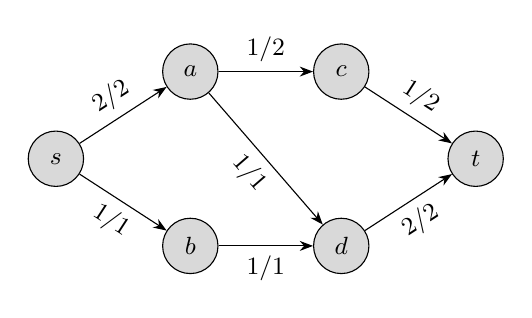
\begin{tikzpicture}[
      mycircle/.style={
         circle,
         draw=black,
         fill=gray,
         fill opacity = 0.3,
         text opacity=1,
         inner sep=0pt,
         minimum size=20pt,
         font=\small},
      myarrow/.style={-Stealth},
      node distance=0.6cm and 1.2cm
      ]
      \node[mycircle] (c1) {$s$};
      \node[mycircle,below right=of c1] (c2) {$b$};
      \node[mycircle,right=of c2] (c3) {$d$};
      \node[mycircle,above right=of c1] (c4) {$a$};
      \node[mycircle,right=of c4] (c5) {$c$};
      \node[mycircle,below right=of c5] (c6) {$t$};

 \foreach \i/\j/\txt/\p in {% start node/end node/text/position
      c1/c2/\text{1/1} /below,
      c1/c4/\text{2/2}/above,
      c2/c3/\text{1/1}/below,
      c3/c6/\text{2/2}/below,
      c4/c5/\text{1/2}/above,
      c5/c6/\text{1/2}/above,
      c4/c3/\text{1/1}/below}
       \draw [myarrow] (\i) -- node[sloped,font=\small,\p] {\txt} (\j);
    \end{tikzpicture}
    
    Take $e_0 = (d, t)$, we can get $N' = N$ except $c'(e_0) = c(e_0) - 1$ with max flow $|f'| = 3$: \\
    
    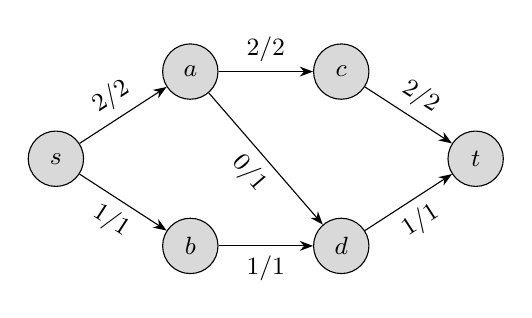
\begin{tikzpicture}[
      mycircle/.style={
         circle,
         draw=black,
         fill=gray,
         fill opacity = 0.3,
         text opacity=1,
         inner sep=0pt,
         minimum size=20pt,
         font=\small},
      myarrow/.style={-Stealth},
      node distance=0.6cm and 1.2cm
      ]
      \node[mycircle] (c1) {$s$};
      \node[mycircle,below right=of c1] (c2) {$b$};
      \node[mycircle,right=of c2] (c3) {$d$};
      \node[mycircle,above right=of c1] (c4) {$a$};
      \node[mycircle,right=of c4] (c5) {$c$};
      \node[mycircle,below right=of c5] (c6) {$t$};

 \foreach \i/\j/\txt/\p in {% start node/end node/text/position
      c1/c2/\text{1/1} /below,
      c1/c4/\text{2/2}/above,
      c2/c3/\text{1/1}/below,
      c3/c6/\text{1/1}/below,
      c4/c5/\text{2/2}/above,
      c5/c6/\text{2/2}/above,
      c4/c3/\text{0/1}/below}
       \draw [myarrow] (\i) -- node[sloped,font=\small,\p] {\txt} (\j);
    \end{tikzpicture}
    
    Thus, $|f^*| = |f'|$.\\
    The statement that $|f'| < |f^*|$ is false.  \\[2ex]
    
    
    \item $Algorithm: $\\
        Denote $e_0$ as $(u_0, v_0)$
        \begin{enumerate}
            \item Do a BFS on the residual network $R$ of $N$ with $f^*$, starting from $u_0$\\
            \item If a path $u_0 \rightarrow v_0$ is found, then construct $f'$ for $N'$ as follows and return $f'$:\\
                $f' = f^*$ except that $f'(u,v) = f^*(u, v) - 1$ for each $(v, u)$ on the path $u_0 \rightarrow v_0$ and $f'(u,v) = f^*(u, v) + 1$ for each $(u, v)$ on the path $u_0 \rightarrow v_0$ in $R$. $f'(u_0, v_0) = f^*(u_0, v_0) - 1$.\\
            \item If no path from $u_0$ to $v_0$ is found, then do a BFS on $R$ start from $t$ to find a path $t\rightarrow v_0$ and do a BFS on $R$ start from $u_0$ to find a path $u_0 \rightarrow s$, so we get a path $t \rightarrow s = t\rightarrow v_0 \rightarrow u_0 \rightarrow s$.
            \item Construct $f'$ for $N'$ as follows and return $f'$: \\
                $f' = f^*$ except that $f'(u, v) = f^*(u, v) - 1$ for each $(v, u)$ on the path $t\rightarrow s$ found in $(iii)$.
        \end{enumerate}
    
    \begin{proof}
    $Proposition:$ For a positive flow $f$ of network $N$, an edge $e$ is contained in some cycle or some $s\rightarrow t$ path in $f$ if $f(e) > 0$.\\
    Justification: If $e = (u, v)$ is in some cycle in $f$, then proof is done. If not, since both of its endpoints satisfy $f^{in} = f^{out}$, $e$ must be connected to an incoming edge $e_1 = (u_1, u)$ for $u$ and an outgoing edge $e_2 = (v, v_1)$ for $v$, both with positive flow equal to $f(e)$. Since $e$ is not contained in any cycle, then $u_1, u, v, v_1$ all distinct.\\
    We can have similar argument for the edges $e_1, e_2$, and find that $u_1$ must be connected to an incoming edge $(u_2, u_1)$ and $v_1$ must be connected to an outgoing edge $(v_1, v_2)$, $u_2, u_1, u, v, v_1, v_2$ all distinct, and so on. \\
    Since there are finite edges and vertices in the network, we can not infinitely extend this path containing $e$, and since no cycle should be created, this path will finally connect to $s, t$, where the incoming flow and outgoing flow do not need to be balanced. \\[2ex]
    
    Proof for algorithm:\\
    Consider the result of the BFS in step 1:\\
    \textbf{Case 1}: A path $p = u_0 \rightarrow v_0$ is found, then $e_0$ is contained in some cycle $p_0 \cup \{(v_0, u_0)\}$ in the residual network $R$. \\
    Since $N'$ is constructed from $N$ by decreasing the capacity of $e_0$, then $|f'| \leq |f^*|$.\\
    Claim that $f'$ is a valid flow with $|f'| = |f^*|$ in this case, then $f'$ is the max flow of $N'$.\\[2ex]
    Justification for the claim: \\
    Denote the cycle $p_0 \cup \{(v_0, u_0)\}$ as $C$.\\
    First show $f'$ is valid. For each node $u$ on $C$, denote its outgoing edge and incoming edge on $C$ as $(v_1, u)$ and $(u, v_2)$, $v_1 \neq v_2$.\\
    If $(v_1, u)$ is in $f^*$, we let $f'(v_1, u) = f^*(v_1, u) + 1$. Otherwise, $(u, v_1)$ is in $f^*$, we let $f'(u, v_1) = f^*(u, v_1) - 1$. If $(u, v_2)$ is in $f^*$, we let $f'(u, v_2) = f^*(u, v_2) + 1$. Otherwise, $(v_2, u)$ is in $f^*$, we let $f'(v_2, u) = f^*(v_2, u) - 1$. Then\\
    For the case $(v_1, u)$ and $(u, v_2)$ in $f^*$, we increase both $f^{in}$ and $f^{out}$ of $u$ by 1.\\
    For the case $(v_1, u)$ and $(v_2, u)$ in $f^*$, we move one flow from $(v_1, u)$ to $(v_2, u)$ and does not change the total flow into $u$.\\
    For the case $(u, v_1)$ and $(u, v_2)$ in $f^*$, we move one flow from $(u, v_1)$ to $(u, v_2)$ and does not change the total flow out from $u$.\\
    For the case $(u, v_1)$ and $(v_2, u)$ in $f^*$, we decrease both $f^{in}$ and $f^{out}$ of $u$ by 1.\\
    Thus, $f^{in}(u) = f^{out}(u)$, i.e. each node is balanced. Also, since we increase/decrease flow of edges according to positive edges in the residual network, we won't get $f < 0$ or $f > c$. \\
    Then show $|f'| = |f^*|$. If $C$ does not contain $s, t$, there is no change to the flow outgoing from $s$ and the flow incoming to $t$. If $C$ contains $s$ or $t$, since $C$ is a cycle, then the algorithm decreases the flow of an outgoing (/incoming) edge of $s$(/$t$) by 1 and increases the flow of another outgoing (/incoming) edge of $s$(/$t$) by 1. Thus, there is no change to  $f_{out}(s)$ and $f_{in}(t)$, and $|f'| = f_{in}(t) = f_{out}(s) = |f^*|$. \\[2ex]
    
    \textbf{Case 2}: If no $u_0 \rightarrow v_0$ path is found, i.e. $e_0$ is not contained in any cycle in $R$, then $e_0$ is not contained in any cycle of $f^*$. (Otherwise, if there is a cycle $v_0 \rightarrow v_1 \rightarrow ... \rightarrow v_m \rightarrow u_0 \rightarrow v_0$ in $f^*$, then we can find cycle $u_0 \rightarrow v_m \rightarrow ... \rightarrow v_1 \rightarrow v_0 \rightarrow u_0$ in $R$).\\
    Then by proposition, $e_0$ is contained in some path $s\rightarrow u_0 \rightarrow v_0 \rightarrow t$ in $f^*$, and thus in path $t\rightarrow v_0 \rightarrow u_0 \rightarrow s$ in $R$. \\[2ex]
    Denote the path found by BFS in $R$ as $P_R$ and the path corresponding to $P_R$ in $f^*$ as $P$\\
    Since we decrease the flow of each edge on $P$ by one, then $f'_{in} = f'_{out}$ for each node on $P$ (except $s,t$). By similar argument to case 1, $f'$ is a valid flow. And $|f'| = f'_{ out}(s) = f^*_{out}(s) - 1 = |f^*| - 1$. Show that this is the max flow on $N'$ by contradiction.\\[2ex]
    Assume that $f'$ is not the max flow, then we can find an augmenting path $P_a$ from $s$ to $t$. \\
    It is obvious that $P_a$ does not contain $e_0$, otherwise, $f'(e_0) < c'(e_0)$ contradiction.\\
    If $P_a \cap P = \emptyset$, i.e. $P_a, P$ do not have common edge, then can find an augmenting path in $N$ with $f^*$, since $f'(e) = f^*(e)$ for each edge $e$ in $P_a$, contradicting that $f^*$ is the max flow of $N$.\\
    If $\exists (x, y) \in P_a \cap P$. If $(x, y) \in$ path $v\rightarrow t$, then we can find a cycle: $s \rightarrow x \rightarrow v \rightarrow u \rightarrow s$ in the residual network $R$,  since in $N$ with $f^*$, edges on the path $s\rightarrow x$ has $f^* < c$ and edges on $s \rightarrow u \rightarrow v \rightarrow x$ has $f^* > 0$.  If $(x, y) \in s\rightarrow x$, then, similarly,  we can find a cycle  $t \rightarrow v \rightarrow u \rightarrow y \rightarrow t$ in the residual network $R$.\\
    Contradicts that there is no cycle in $R$.\\
    Thus, $f'$ is the maxflow in this case and $|f'| = |f^*| - 1$.\\
    \end{proof}
    
    $Complexity: $\\
    For step (i), constructing residual network and doing a BFS both take $\mathcal{O}(|E| + |V|)$ time.\\
    If $e_0$ is in a cycle, for step (ii), reducing/increasing flow of edges on a cycle takes $\mathcal{O}(|V|)$ time.\\
    If $e_0$ is not in a cycle, For step (iii), two BFS take $\mathcal{O}(|E| + |V|)$ time. For step (iv), reducing/increasing flow of edges on a path takes $\mathcal{O}(|V|)$ time.\\
    Thus, the algorithm runs in $\mathcal{O}(|E| + |V|) + max\{ \mathcal{O}(|V|), \mathcal{O}(|E| + |V|)  + \mathcal{O}(|V|\}$ time, i.e. $\mathcal{O}(|E| + |V|)$ time.\\[2ex]
    
    \item $Algorithm$:\\
    \begin{enumerate}
        \item Initialize an empty list $L$ for storing the edges satisfying the condition
        \item Find a max flow $f^*$ of $N$ (using Edmonds-Karp algorithm)
        \item Construct the residual network $R$ of $N$ with $f^*$.
        \item For each edge $e = (u, v)$ in $N$, if $f^*(e) < c(e)$, continue to the next edge.\\
        Otherwise, run a BFS on the residual network $R$ of $N$ with $f^*$, starting from $v$.\\
        If $e$ is not contained in any cycle in $R$, add $e$ to $L$. 
        \item return $L$\\[2ex]
    \end{enumerate}
    $Correctness: $
    \begin{proof}
        The correctness for BFS and Edmonds-Karp algorithm is shown in textbook.\\
        The way of constructing the residual network is shown in class and we assume its correctness.\\
        For the iteration step (step (iv)), consider edge $e = (u, v)$:\\
        \textbf{Case 1}: If $f^*(e) < c(e)$, then we can decrease $c(e)$ by one without affecting the flow through $e$ and the whole network. Thus $e$ is not the edge we want and the algorithm does not add it to the result list.\\
        \textbf{Case 2}: If $f^*(e) = c(e)$, then we run BFS on the residual network $R$ of $N$ with $f^*$. \\
        By the proof for part(b), we know that if the corresponding $e_R = (v, u)$ (no forward edge since c - f = 0) in $R$ of $e$ is in some cycle in $R$, then we can find $f'$ on $N' = N$ except $c'(e) = c(e) - 1$, s.t. $|f'| = |f^*|$, thus, decreasing the capacity of $e$ by one unit will not affect the value of max flow and the algorithm won't add $e$ to result list.\\
        If $e_R$ is not in any cycle in $R$, then max flow $f'$ on $N' = N$ except $c'(e) = c(e) - 1$ has $|f'| = |f^*| - 1$. Then decreasing the capacity of $e$ by one unit will cause the value of max flow to decrease and the algorithm will add $e$ to result list.\\
        Thus, after looping over all edges in $N$, the result list $L$ contains all the edges as we want.
    \end{proof}
    
    $Complexity: $\\
    Step (i) and (v) takes constant time.\\
    Step (ii) solves the max flow problem using Edmonds-Karp algorithm, which takes $\mathcal{O}(|V||E|^2)$. \\
    Step (iii) constructing the residual network takes the time to copy the set of vertices of $N$, and a constant time at each edge in $N$ to construct the corresponding forward and backward edge in $R$. Thus in $\mathcal{O}(|V||E|)$ time.\\
    For the iteration over step (iv), each iteration takes the time of a BFS, i.e. $\mathcal{O}(|E| + |V|)$, at edge with $f^* = c$; and takes constant time at edge with $f^* < c$. Then the total runtime of the loop is $\mathcal{O}(|E|^2 + |E||V|)$ time.\\
    Thus, the algorithm takes a total of $\mathcal{O}(|V||E|^2 + |E|^2 + |E||V|)$ = $\mathcal{O}(|V||E|^2)$ time.
    
 \end{enumerate}
\end{enumerate}


\end{document}
